% $Header: /home/vedranm/bitbucket/beamer/solutions/generic-talks/generic-ornate-15min-45min.en.tex,v 90e850259b8b 2007/01/28 20:48:30 tantau $

\documentclass{beamer}

% This file is a solution template for:

% - Giving a talk on some subject.
% - The talk is between 15min and 45min long.
% - Style is ornate.



% Copyright 2004 by Till Tantau <tantau@users.sourceforge.net>.
%
% In principle, this file can be redistributed and/or modified under
% the terms of the GNU Public License, version 2.
%
% However, this file is supposed to be a template to be modified
% for your own needs. For this reason, if you use this file as a
% template and not specifically distribute it as part of a another
% package/program, I grant the extra permission to freely copy and
% modify this file as you see fit and even to delete this copyright
% notice.


\mode<presentation>
{
  \usetheme{Warsaw}
  % or ...

  \setbeamercovered{transparent}
  % or whatever (possibly just delete it)
}

      \newtheorem{proposition}[theorem]{Proposition}
      \theoremstyle{definition}
      \newtheorem{game}[theorem]{Game}
      \newtheorem{question}[theorem]{Question}

\usepackage[english]{babel}
% or whatever

\usepackage[latin1]{inputenc}
% or whatever

\usepackage{times}
\usepackage[T1]{fontenc}
% Or whatever. Note that the encoding and the font should match. If T1
% does not look nice, try deleting the line with the fontenc.


\usepackage{marvosym} % For \Smiley
\usepackage{verbatim} % for \verbatiminput

\usepackage{tikz}
\usetikzlibrary{matrix} % for diagrams

\title
{Limited information strategies for topological games}

\subtitle
{PhD Defense} % (optional)

\author%[Author, Another] % (optional, use only with lots of authors)
{Steven~Clontz~http://stevenclontz.com}%\inst{1} \and S.~Another\inst{2}}
% - Use the \inst{?} command only if the authors have different
%   affiliation.

\institute[Auburn University] % (optional, but mostly needed)
{
  %\inst{1}%
  Department of Mathematics and Statistics\\
  Auburn University}
  %\and
  %\inst{2}%
  %Department of Theoretical Philosophy\\
  %University of Elsewhere}
% - Use the \inst command only if there are several affiliations.
% - Keep it simple, no one is interested in your street address.

\date[15-03-11] % (optional)
{March 11, 2015}


% If you have a file called "university-logo-filename.xxx", where xxx
% is a graphic format that can be processed by latex or pdflatex,
% resp., then you can add a logo as follows:

 % \pgfdeclareimage[height=1cm]{university-logo}{auburn_logo.png}
 % \logo{\pgfuseimage{university-logo}}



% Delete this, if you do not want the table of contents to pop up at
% the beginning of each subsection:
%\AtBeginSubsection[]
%{
%  \begin{frame}<beamer>{Outline}
%    \tableofcontents[currentsection,currentsubsection]
%  \end{frame}
%}


% If you wish to uncover everything in a step-wise fashion, uncomment
% the following command:

%\beamerdefaultoverlayspecification{<+->}

% Strategy uparrow shortcuts
\newcommand{\win}{\uparrow}
\newcommand{\prewin}{\underset{\text{pre}}{\uparrow}}
\newcommand{\markwin}{\underset{\text{mark}}{\uparrow}}
\newcommand{\tactwin}{\underset{\text{tact}}{\uparrow}}
\newcommand{\kmarkwin}[1]{\underset{#1\text{-mark}}{\uparrow}}
\newcommand{\ktactwin}[1]{\underset{#1\text{-tact}}{\uparrow}}
\newcommand{\codewin}{\underset{\text{code}}{\uparrow}}
\newcommand{\limitwin}{\underset{\text{limit}}{\uparrow}}
\newcommand{\notwin}{\not\uparrow}
\newcommand{\notprewin}{\underset{\text{pre}}{\not\uparrow}}
\newcommand{\notmarkwin}{\underset{\text{mark}}{\not\uparrow}}
\newcommand{\nottactwin}{\underset{\text{tact}}{\not\uparrow}}
\newcommand{\notkmarkwin}[1]{\underset{#1\text{-mark}}{\not\uparrow}}
\newcommand{\notktactwin}[1]{\underset{#1\text{-tact}}{\not\uparrow}}
\newcommand{\notcodewin}{\underset{\text{code}}{\not\uparrow}}
\newcommand{\notlimitwin}{\underset{\text{limit}}{\not\uparrow}}

\newcommand{\oneptcomp}[1]{#1^*}
\newcommand{\oneptlind}[1]{#1^\dagger}
% \newcommand{\sharp}[1]{#1^{\#}}

% Games
\newcommand{\gruConGame}[2]{Gru_{O,P}^{\to}\left({#1},{#2}\right)}
\newcommand{\gruConGameHard}[2]{Gru_{O,P}^{\to,\star}\left({#1},{#2}\right)}
\newcommand{\gruClusGame}[2]{Gru_{O,P}^{\leadsto}\left({#1},{#2}\right)}
\newcommand{\gruClusGameHard}[2]{Gru_{O,P}^{\leadsto,\star}\left({#1},{#2}\right)}

\newcommand{\gruKPGame}[1]{Gru_{K,P}\left({#1}\right)}
\newcommand{\gruKLGame}[1]{Gru_{K,L}\left({#1}\right)}

\newcommand{\cloPFGame}[1]{PtFin_{F,C}\left({#1}\right)}

\newcommand{\menGame}[1]{Men_{C,F}\left({#1}\right)}
\newcommand{\rothGame}[1]{Roth_{C,S}\left({#1}\right)}
\newcommand{\rothAltGame}[1]{Roth_{P,O}\left({#1}\right)}

\newcommand{\cloFillStrictGame}[1]{Fill^{\cup,\subset}_{C,F}\left({#1}\right)}
\newcommand{\cloFillGame}[1]{Fill^{\cup,\subseteq}_{C,F}\left({#1}\right)}
\newcommand{\cloFillInitialGame}[1]{Fill^{1,\subseteq}_{C,F}\left({#1}\right)}
\newcommand{\cloFillIntGame}[1]{Fill^{\cap}_{C,F}\left({#1}\right)}

\newcommand{\bellUniGame}[1]{Bell_{D,P}^{\textrm{uni}}\left({#1}\right)}
\newcommand{\bellConGame}[1]{Bell_{D,P}^{\rightharpoonup}\left({#1}\right)}
\newcommand{\bellConHardGame}[1]{Bell_{D,P}^{\rightharpoonup,\star}\left({#1}\right)}
\newcommand{\bellAbsConGame}[1]{Bell_{D,P}^{\to}\left({#1}\right)}
\newcommand{\bellAbsConHardGame}[1]{Bell_{D,P}^{\to,\star}\left({#1}\right)}



\newcommand{\SigmaProdR}[1]{\Sigma\mathbb{R}^{#1}}
\newcommand{\sigmaprodtwo}[1]{\Sigma2^{#1}}

\newcommand{\concat}{{^\frown}}
\newcommand{\rest}{\restriction}

\newcommand{\cl}[1]{\overline{#1}}

\newcommand{\pow}[1]{\mc{P}(#1)}

\newcommand{\<}{\langle}
\renewcommand{\>}{\rangle}

\newcommand{\al}[1]{{#1}^*}

\newcommand{\mc}[1]{\mathcal{#1}}
\newcommand{\mb}[1]{\mathbb{#1}}

\newcommand{\po}{\mathbb{P}}
\newcommand{\pok}{\po_\kappa}

\newcommand{\Lim}{\mathrm{Lim}}
\newcommand{\Suc}{\mathrm{Suc}}

\newcommand{\ds}{\displaystyle}

\newcommand{\st}[2]{st\left(#1,#2\right)}

\newcommand{\alcomp}{\al\parallel}

\newcommand{\rank}{\textrm{rank}}
\newcommand{\dom}{\textrm{dom}}

\renewcommand{\mod}{\,\textrm{mod}}

\newcommand{\zip}{\bowtie}
\newcommand{\ran}[1]{\text{range}(#1)}

\newcommand{\cf}[1]{\textrm{cf}(#1)}

\newcommand{\alcompS}[1]{S(#1)}


\newcommand{\scish}{almost-$\sigma$-(relatively compact)}

\usepackage{mathrsfs}
\newcommand{\pl}[1]{\mathscr{#1}}



\newcommand{\term}{\textit}


\newcommand{\bmGame}[1]{{BM}_{E,N}(#1)}





\begin{document}
\renewcommand{\pause}{}
\newcommand{\vspacing}{\vspace{1em}}
\newcommand{\vpause}{\pause\vspacing}

\begin{frame}
  \titlepage
\end{frame}

\section{Topological Games}

\subsection{Defintion}

\begin{frame}
  A \term{topological game} is a two-player game $G(X)$ of length
  $\omega=\{0,1,2,\dots\}$ defined for certain topological spaces $X$.

  \vpause

  During each round $n$, the first and second player take turns choosing
  certain topological objects from $X$ (e.g. point, open set, open cover, etc.).

  \vpause

  At the ``end'' of the game, a winner is declared by inspecting the sequences
  of choices made throughout the game.

  \vpause

  The study of such games involves finding when a player has a
  \term{winning strategy} which defeats every possible counterattack by
  the opponent.

  \vpause

  {\tiny See Telgarsky's excellent survey on topological games for more
  details: \cite{MR892457}}
\end{frame}

\subsection{Example}

\begin{frame}
  \small
  \begin{game}
    The \term{Banach-Mazur Game}
    $\bmGame{X}$ (1935) \cite{MR666400}

    \begin{figure}
      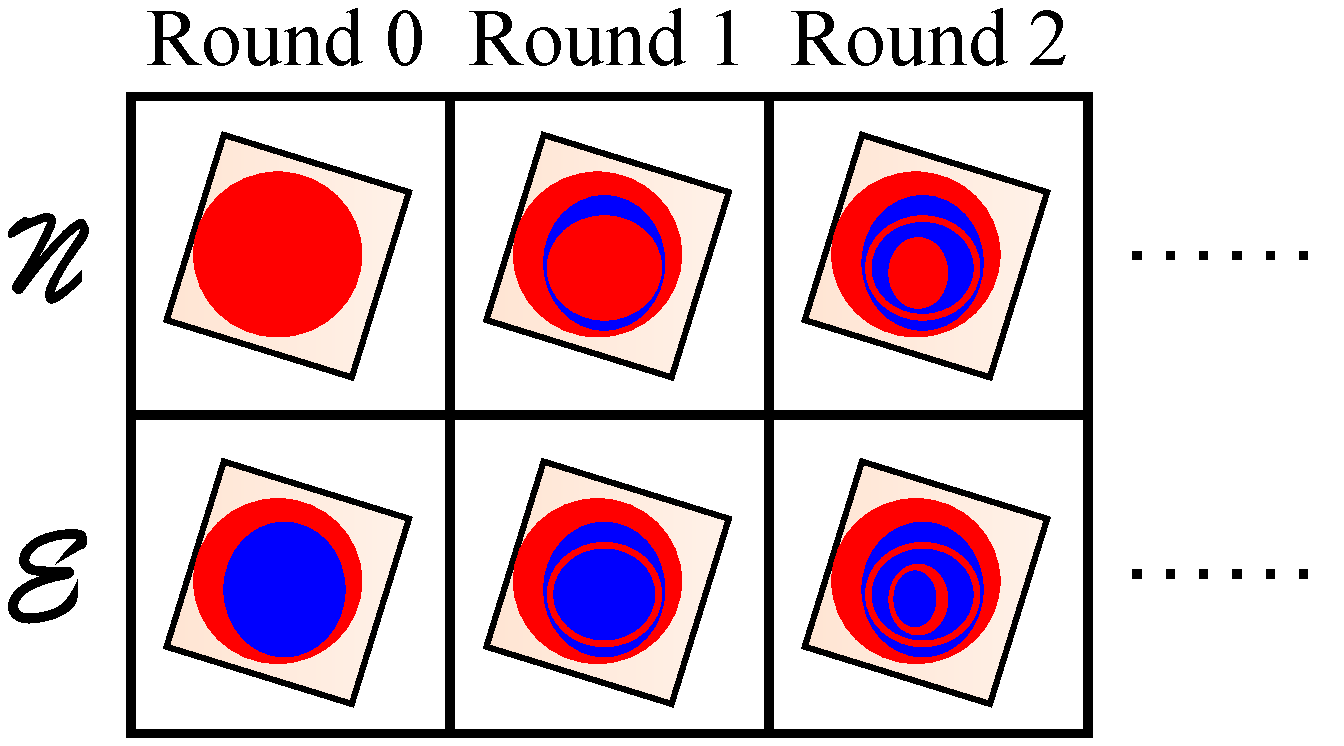
\includegraphics[width=0.6\linewidth]{bmGame.pdf}
    \end{figure}

  The first player $\pl N$ wins the game if the intersection of all the chosen
  open sets is nonempty.
  \end{game}
\end{frame}

\begin{frame}
  \begin{theorem}
    $X$ is Baire if and only if $\pl N$ lacks a winning strategy
    in the Banach Mazur game ($\pl N\not\win\bmGame{X}$).
  \end{theorem}

  \pause

  Thus the topological property of being a Baire space has a game-theoretic
  characterization using $\bmGame{X}$.

  \vpause

  By considering \term{limited information strategies}, we may characterize
  more properties.
\end{frame}

\begin{frame}
  Consider the following:

  \begin{theorem}
    $X$ is $\alpha$-favorable $\Rightarrow$
    $X$ is weakly $\alpha$-favorable $\Rightarrow$
    $X$ is Baire
  \end{theorem}

  \pause

  $\alpha$-favorability is characterized by $\pl E\tactwin\bmGame{X}$:
  player $\pl E$ has a \term{tactical} winning strategy which only considers
  the most recent move of the opponent.

  \vpause

  This is stronger than weak
  $\alpha$-favorability, characterized by $\pl E\win\bmGame{X}$.
  In this case $\pl E$ still has a winning strategy, but it may
  rely on perfect information of the history of the game.
\end{frame}

\subsection{Motivation}

\begin{frame}
  By characterizing topological properties using the theory of
  topological games, we introduce new proof techniques for demonstrating
  the structure of given topological spaces.

  \vpause

  The aim of my dissertation was to investigate four topological games
  from the literature with unknown limited information implications.

  \vpause

  In doing so I uncovered several new results in general topology,
  advancing research done by
  G. Gruenhage, P. Nyikos, R. Telg{\' a}rksy, J. Bell,
  M. Scheepers, and others.
\end{frame}

\section{Gruenhage's Convergence/Clustering Games}

\subsection{Definition}

\begin{frame}
  \small
  \begin{game}
  Gruenhage's convergence game $\gruConGame{X}{x}$
  and clustering game $\gruClusGame{X}{x}$ proceed as follows:
    \begin{figure}
      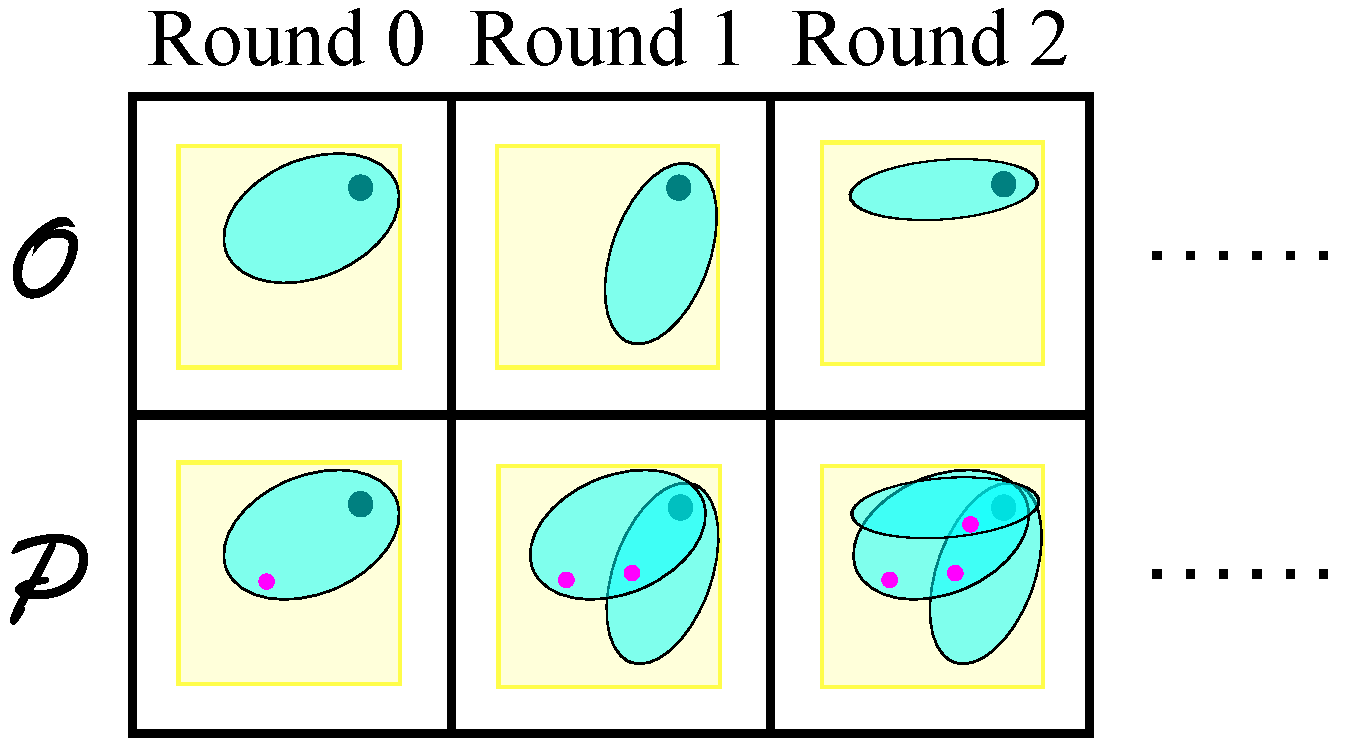
\includegraphics[width=0.6\linewidth]{convergenceGame.pdf}
    \end{figure}

  $\pl O$ wins the game if the points chosen by $\pl P$ converge/cluster
  to the given point $x\in X$. Otherwise, $\pl P$ wins.
  \end{game}

  \tiny
  Note that $\pl O$ need not know anything about the history of the game
  to play each round.
\end{frame}

\subsection{Motivation}

\begin{frame}
  If $\pl O\win \gruConGame{X}{x}$, then $x$ is called a $W$-point in $X$.
  Obviously, all points of first-countablity are $W$-points, but
  $\pl O\win\gruConGame{\oneptcomp\kappa}{\infty}$ also, where $\infty$
  is the added point in the one-point compactification $\oneptcomp\kappa$
  of uncountable discrete $\kappa$.

  \vpause

  Points of first-countability may in fact be characterized by this game
  as well:
  \begin{theorem}
    $x$ has a countable local base in $X$ if and only if
    $\pl O\prewin \gruConGame{X}{x}$ ($\pl O$ has
    a winning \term{predetermined}
    strategy using only the round number).
  \end{theorem}

  \pause

  If every point in a space $X$ is a $W$-point, then $X$ is a $W$-space.
\end{frame}

\subsection{Results}

\begin{frame}
  A variation of this game which is harder for $\pl O$ yields some
  difficult infinite combinatorial questions:

  \begin{game}
  Gruenhage's hard convergence game $\gruConGameHard{X}{x}$
  and hard clustering game $\gruClusGameHard{X}{x}$ proceed as follows:
    \begin{figure}
      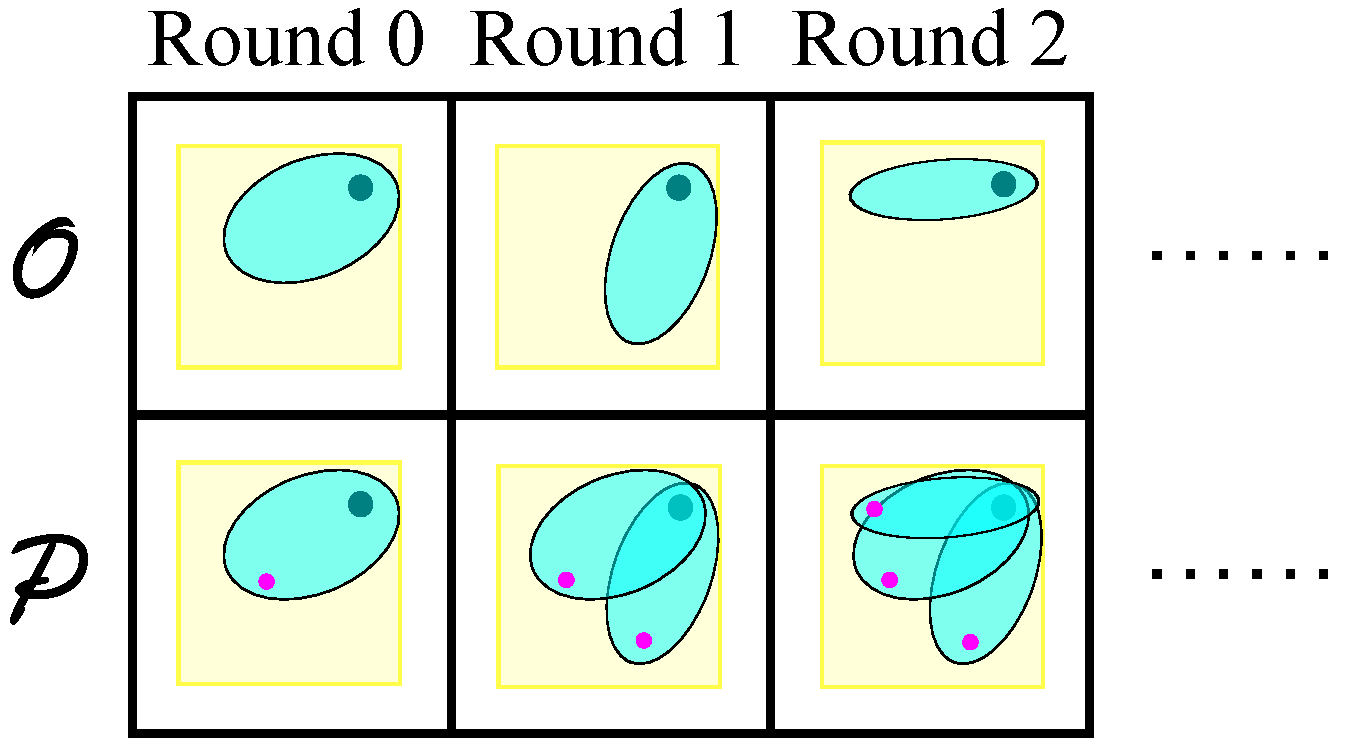
\includegraphics[width=0.6\linewidth]{convergenceHardGame.pdf}
    \end{figure}
  \end{game}
\end{frame}

\begin{frame}
  Nyikos observed in \cite{MR1031771} that:
  \begin{theorem}
    $\pl O \notmarkwin \gruConGameHard{\oneptcomp\omega_1}{\infty}$.

    {\small ($\pl O$ cannot guarantee a win using a \term{Markov strategy}
    which considers only the round number and most recent move.) }
  \end{theorem}

  \vpause

  Some more work shows that in fact
  \begin{theorem}
    $\pl O \notkmarkwin{k} \gruConGameHard{\oneptcomp\omega_1}{\infty}$.

    {\small ($\pl O$ cannot guarantee a win using a $k$-\term{Markov strategy}
    which considers only the round number and $k$ most recent moves.) }
  \end{theorem}
\end{frame}


\begin{frame}
  Interestingly, the strategy which prevents convergence won't
  prevent clustering as well unless the cardinality of the space is
  sufficiently large.

  \begin{theorem}
    $\pl O\markwin \gruClusGameHard{\oneptcomp\omega_1}{\infty}$, but
    $\pl O\notkmarkwin{k}\gruClusGameHard{\oneptcomp\omega_2}{\infty}$.
  \end{theorem}

  \pause

  But knowledge of the round number is used non-trivially in doing so.

  \begin{theorem}
    $\pl O\notktactwin{k}\gruClusGameHard{\oneptcomp\omega_1}{\infty}$.
  \end{theorem}
\end{frame}




\section{Bell's Proximal Game}

\subsection{Definition}

\begin{frame}
  \small
  \begin{game}
  Bell's proximal game $\bellAbsConGame{X}$ for compact zero-dimensional
  $X$:
    \begin{figure}
      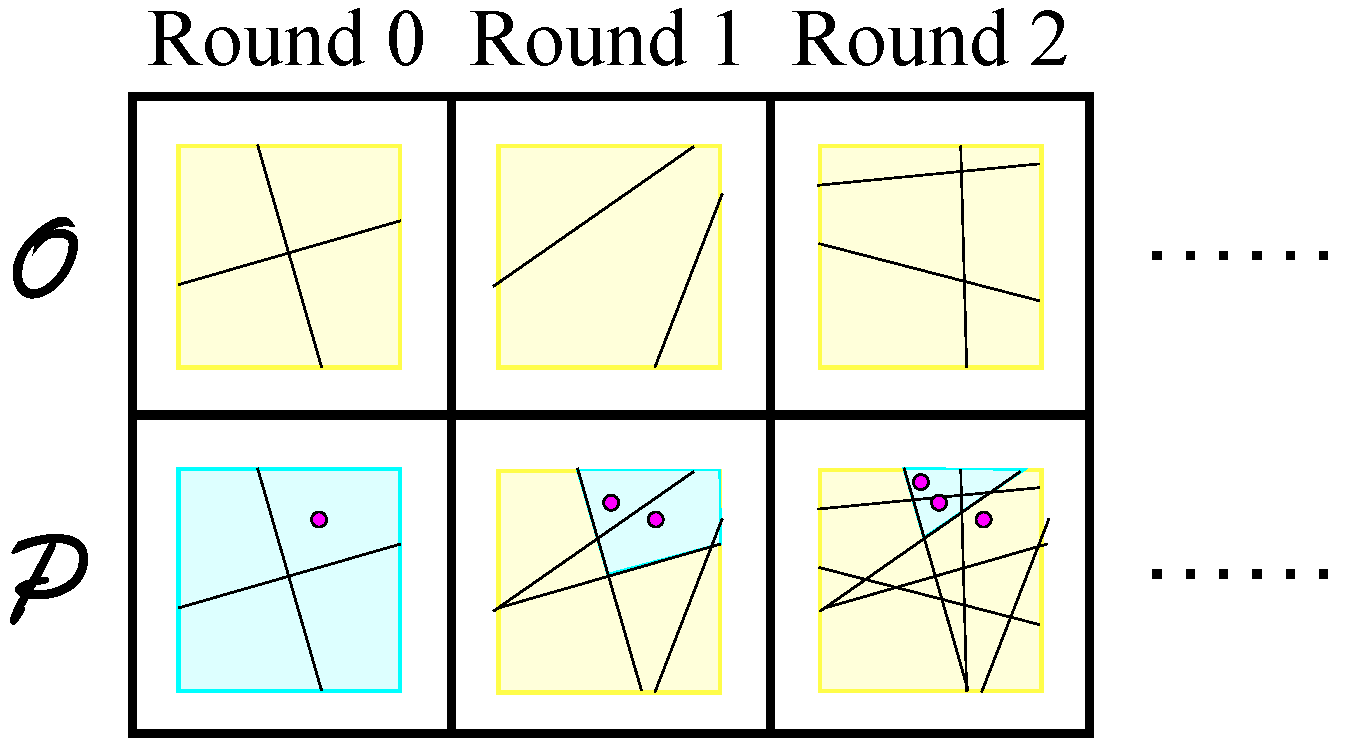
\includegraphics[width=0.6\linewidth]{proximalGameAlt.pdf}
    \end{figure}

  $\pl D$ wins the game if the points chosen by $\pl P$ converge.
  Otherwise, $\pl P$ wins.
  \end{game}
\end{frame}

\subsection{Motivation}

\begin{frame}
  If $\pl D\win \bellAbsConGame{X}$, then $X$ is called a proximal compact.
  This game was brought to my attention due to this result: \cite{MR3239205}

  \begin{theorem}
    Every proximal space is a $W$-space. So
    $\pl D\win\bellAbsConGame{X} \Rightarrow \pl O\win\gruConGame{X}{x}$
    for all $x\in X$.
  \end{theorem}

  \vpause

  Proximal spaces have strong preservation properties, as any
  closed subset or $\Sigma$-product of proximal spaces is proximal. Since
  any proximal space is collectionwise normal, Bell's game gives an elegant
  proof of the classic result:

  \begin{theorem}
    A $\Sigma$-product of metrizable spaces is collection-wise normal.
  \end{theorem}
\end{frame}

\subsection{Results}

\begin{frame}
  Nyikos \cite{nyikosProximalPreprint} observed that
  \begin{proposition}
    Corson compact spaces are proximal.
  \end{proposition}
  and asked if the converse holds as well.

  \vpause

  With Gruenhage, I showed that the answer is yes:
  \begin{theorem}
    A compact space is Corson compact if and only if it is proximal.
  \end{theorem}
\end{frame}

\begin{frame}\small
  A winning limited information strategy may always be passed down
  to win in a closed subspace, but Bell's result that winning strategies
  are preserved for $\Sigma$-products does not quite generalize as well:

  \begin{theorem}
    For $k<\omega$, if $\pl D\kmarkwin{k}\bellAbsConGame{X_i}$ for all $i<\omega$,
    then $\pl D\kmarkwin{k}\bellAbsConGame{\prod_{i<\omega} X_i}$.
  \end{theorem}

  \pause

  Other limited information lemmas proved in my dissertation allowed me
  to prove a game-theoretic characterization of another compactness property
  (paper in preparation):

  \begin{theorem}
    A compact space is strong Eberlein compact if and only if
    $\pl D\tactwin\bellAbsConGame{X}$.
  \end{theorem}
\end{frame}





\section{Gruenhage's Locally Finite Games}

\subsection{Definition}

\begin{frame}
  \small
  \begin{game}
  Gruenhage's locally finite games $\gruKPGame{X}$ and
  $\gruKLGame{X}$ proceed as follows:
    \begin{figure}
      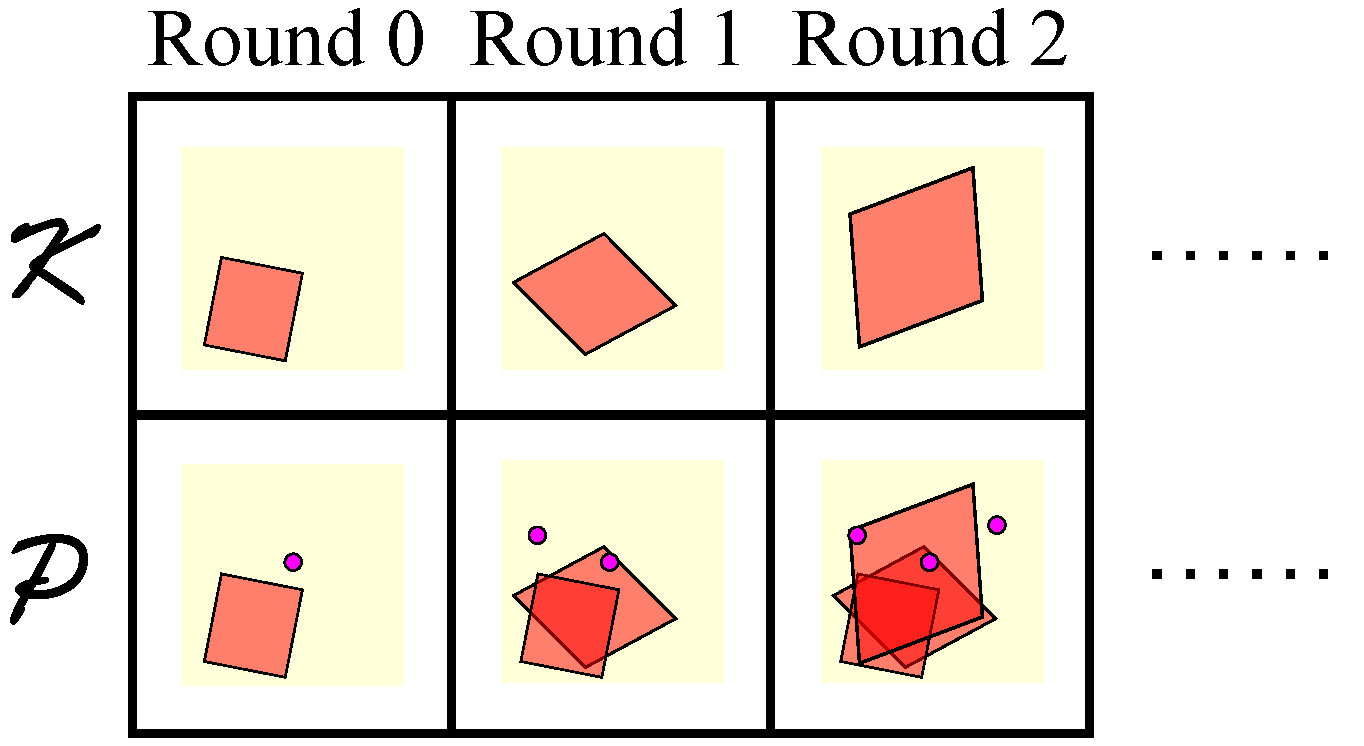
\includegraphics[width=0.6\linewidth]{compactPointGame.pdf}
    \end{figure}

  $\pl K$ wins the game if the points/sets chosen by $\pl P$/$\pl L$ are
  locally finite in the space. Otherwise, $\pl P$/$\pl L$  wins.
  \end{game}
\end{frame}

\subsection{Motivation}

\begin{frame}
  Gruenhage used these games in \cite{MR752278} to characterize
  metacompactness and $\sigma$-metacompactness amongst locally compact
  spaces:

  \begin{theorem}
    For locally compact spaces, $\pl K\tactwin\gruKPGame{X}$ if and only if
    $X$ is metacompact.
  \end{theorem}

  \begin{theorem}
    For locally compact spaces, $\pl K\markwin\gruKPGame{X}$ if and only if
    $X$ is $\sigma$-metacompact.
  \end{theorem}
\end{frame}

\subsection{Results}

\begin{frame}
  By removing knowledge of the round number, an analogous result is
  unsurfaced:

  \begin{theorem}
    For locally compact spaces, $\pl K\prewin\gruKPGame{X}$ if and only if
    $X$ is $\sigma$-compact.
  \end{theorem}

  \pause

  Actually, for locally compact or even compactly-generated spaces,
  $\pl K\prewin\gruKPGame{X}$ if and only if $\pl K\prewin\gruKLGame{X}$.
  However, there is a non-compactly-generated counterexample:

  \begin{theorem}
    There exists a free ultrafilter $\mc F$ such that
    $\pl K \prewin\gruKPGame{\omega\cup\{\mc F\}}$, but
    $\pl K \notprewin\gruKLGame{\omega\cup\{\mc F\}}$ for any free
    ultrafilter $\mc F$.
  \end{theorem}
\end{frame}





\section{Menger's Game}

\subsection{Definition}

\begin{frame}
  \small
  \begin{game}
  Menger's game $\menGame{X}$ proceeds as follows:

  (this space intentionally left blank until I make a picture)

  $\pl F$ wins the game if her finitely coverable subsets
  union to the space. Otherwise, $\pl C$  wins.
  \end{game}
\end{frame}

\subsection{Motivation}

\begin{frame}
  A covering property generalizing $\sigma$-compactness is characterized
  by this game, demonstrated by Hurewicz in the 1920's. \cite{MR1544773}

  \begin{theorem}
    A space is Menger if and only if $\pl C\not\win\menGame{X}$.
  \end{theorem}

  \pause

  It was originally suspected that Menger subspaces of the real line were
  exactly the $\sigma$-compact subspaces, but as was shown by Telgarsky
  and Scheepers, $\sigma$-compact spaces
  have slightly more structure. \cite{MR753073} \cite{MR1273523}

  \begin{theorem}
    A metrizable space $X$ is $\sigma$-compact if and only if
    $\pl F\win\menGame{X}$.
  \end{theorem}
\end{frame}

\subsection{Results}

\begin{frame}
  By considering Markov strategies, the previous theorem may be factored
  into two subresults.

  \begin{theorem}
    A regular space $X$ is $\sigma$-compact if and only if
    $\pl F\markwin\menGame{X}$.
  \end{theorem}
  \begin{theorem}
    For a second-countable space $X$, $\pl F\win\menGame{X}$ if and only if
    $\pl F\markwin\menGame{X}$.
  \end{theorem}

  Note that since the spaces we are considering are all Lindel\"of,
  metrizability is characterized by regularity and second-countability.
\end{frame}

\subsection{More Motivation}

\begin{frame}
  Limited information strategies in topological games such as
  $\menGame{X}$ often have set-theoretic
  consequences. The statement $\alcompS\kappa$ due to M. Scheepers
  \cite{MR1129143} says that there exist
  almost-compatible functions $f_A:A\to\omega$ for each $A\in[\kappa]^\omega$.

  \begin{theorem}
    $\alcompS{\omega_1}$ and $\neg\alcompS{(2^\omega)^+}$ are theorems
    of $ZFC$, but $\alcompS\kappa$ is independent of $ZFC$ for
    $\omega_1<\kappa\leq 2^\omega$.
  \end{theorem}

  \begin{theorem}
    If $\alcompS{\kappa}$ holds, then
    $\pl F\ktactwin2 \cloFillStrictGame{\kappa}$.
  \end{theorem}
\end{frame}

\subsection{More Results}

\begin{frame}
  Let $\oneptlind\kappa$ be the one-point ``Lindel\"of-ication'' of
  discrete $\kappa$.

  \begin{theorem}
    \begin{figure}
      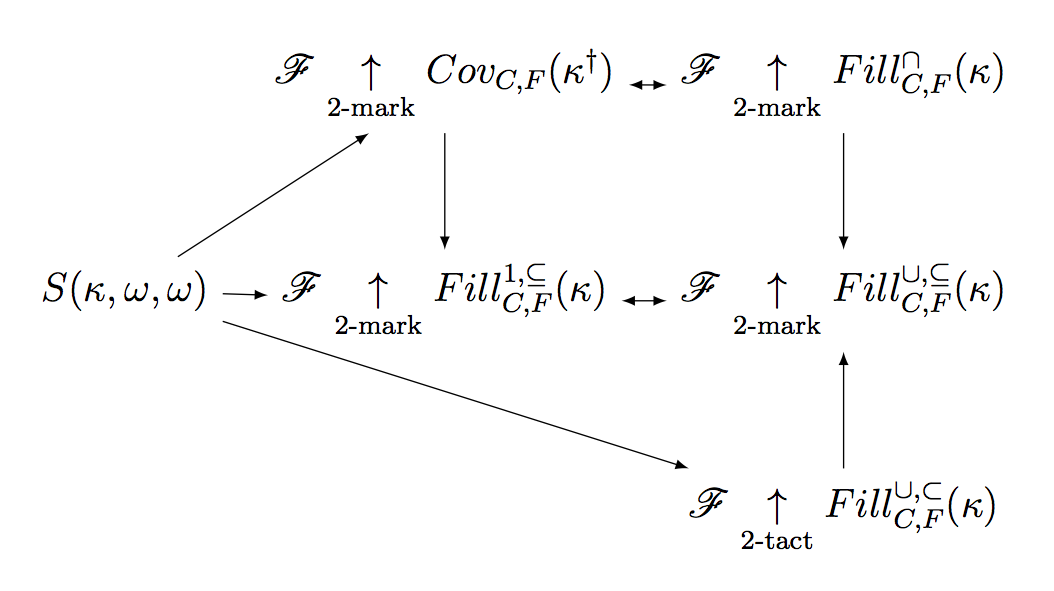
\includegraphics[width=0.6\linewidth]{mengerGameChart.png}
    \end{figure}
  \end{theorem}
\end{frame}

\begin{frame}\small
  For most of the games in the previous chart, including the Menger game
  $\menGame{X}$, there's no need to consider larger amounts of limited
  information.

  \begin{theorem}
    For each $k<\omega$,
    $\pl F\kmarkwin{k+2}\menGame{X}$ if and only if
    $\pl F\kmarkwin2\menGame{X}$
  \end{theorem}

  The topological property $\pl F\kmarkwin2\menGame{X}$ seems to
  depend on the set-theoretic axioms at play.

  \begin{theorem}
    If $\alcompS{2^\omega}$, then $\pl F\kmarkwin2\menGame{R_\omega}$.
  \end{theorem}
\end{frame}


\begin{frame}[allowframebreaks]
  \tiny
  \bibliographystyle{plain}
  \bibliography{../dissertation/bibliography}
\end{frame}

\begin{frame}
  Any questions?
\end{frame}


\end{document}


